\section{New Directions for Mapping between NDA Abstractions}
\label{sec:approaches}

\begin{quote}
{\em The technical community expanded to reach areas of expertise in non-linear and combinatorial optimization, control, artificial intelligence, and logic.} -- The Tides of EDA~\cite{alberto}
\vspace{-2mm}
\end{quote}

The preceding section presented abstractions to address network design and debugging challenges. The utility of these abstractions depends upon methodologies to map between abstraction levels, as in EDA. Some mapping tasks are relatively straightforward, while others are risky, potentially transformative, and some require new science. While the directions are necessarily diverse to address different stakeholders (architects, operators), they are united by common themes: {\em interdisciplinary} (using multiple skill sets enabled by an NSF Large) and {\em domain-specific} (addressing the complexities but exploiting the structure of networks).


\subsection{From Constraints to Wiring: Topology Synthesis}

\paragraph*{Tool:} (Challenge C4, Foster, Govindan). A network
architect must map a specification of a network in terms of
constraints (that reflect both design objectives and resource limits)
into a physical topology of routers and wires ({\bf S4}).
%
\paragraph*{Science:} Past work~\cite{condor} has focused on {\em data
  centers} and {\em connectivity} constraints and used mapping
heuristics; we will generalize to {\em general networks} and {\em
  generic} constraints and map using Counter-Example Guided Inductive
Synthesis (CEGIS).


%early versions focused on
%connectivity~\cite{PA} and structure~\cite{Hongsuda}, and later
%versions explored bandwidth, latency and cost~\cite{HOT}.

\paragraph*{Approach:}
%
Network topologies must balance competing objectives including high
bandwidth, fault tolerance and low cost. Today, designing a large
network topology can take a human expert up to six weeks. Although
modeling and simulation tools are often used as aids, the design
process is still largely done by hand.  While topology design can be
framed as combinatorial optimization~\cite{PA,
  Hongsuda,HOT}, prior work has only been used to {\em understand}
the structure of existing networks and not to {\em design} new ones.

We plan to develop a domain-specific programming language in which
planners may specify constraints on the design.  Our point of
departure is recent work at Google on a domain-specific language (DSL)
for data-center topologies called TDL~\cite{condor}). TDL can be used
to generate a specific class of topologies (Fat-Trees~\cite{FatTree})
whose links and switches are relatively homogeneous, subject to
connectivity constraints between different tiers of the Fat-Tree. We
will design a more general DSL for wide-area networks (WAN) and
enterprise networks that will support more general constraints
essential for these networks such as latency, traffic-carrying
capacity, costs, and limited optical touchdown points available from
optical vendors.

%many more dimensions in the specification language:
%higher-level constraints on end-to-end latency and link capacity
%oversubscriptions, constraints expressing commercially available
%router capabilities and link capacities (since WAN and enterprise
%topologies are constructed from heterogeneous devices and link
%capacities), constraints on the cost of wide-area links, constraints
%that simplify the manageability of the network (e.g., hierarchical
%structure that permits designers to easily visualize network
%structure) and constraints that specify optical touchdown points
%available from optical network providers.  The language will come
%equipped with tools for synthesizing the missing pieces of a design
%and for analyzing its qualities---e.g., a planner may wish to debug a
%design by checking if specific properties are satisfied.

We plan to use Counter-Example Guided Inductive Synthesis
(CEGIS)~\cite{sketch} to search through the space of possible
topologies, learning from counter-examples to quickly rule out
topologies that do not provide required functionality. To make
synthesis tractable, we will need to build tools that can rapidly
answer reachability queries as well as quantitative questions
involving bandwidth and fault tolerance. Finally, we will explore
domain-specific heuristics such as generating topologies from a fixed
class and exploiting its structure and symmetries, inspired by
heuristically-optimal topologies~\cite{HOT}.  We will also explore
synergies with constraint-based approaches used in EDA for high-level
synthesis~(e.g., \cite{cong}).

\iffalse
Finally, we will explore several novel directions in topology
synthesis. Today, the topology planning team at Facebook uses real
data about bandwidth and latency but assumes that the routing is
optimal, when in practice traffic is carried along a relatively small
number of shortest paths. Designing topology with realistic routing
models can result in networks with higher utilization and lower
overall cost.  We also plan to explore how to synthesize topologies
that satisfy all other constraints and are also robust with respect to
expected failure models. This is a step beyond the state of the art in
large providers, who only have tools to determine whether a given
topology can satisfy a given traffic matrix under a given failure
model.\jnf{The distinction between expected failure model vs. given
  failure model being used here is a bit subtle.} Finally, we plan to
explore ways of incrementally augmenting designs in ways that preserve
the original design constraints (or, in addition, new performance
properties) while requiring minimal modifications to the existing
network.


\paragraph*{Task.} (Challenge C2, Foster, Govindan). After designing
router hardware, a network architect must wire routers together to
make a physical network ({\bf S4}).
%

Network topologies are expected to balance a number of competing
factors including high bandwidth, low latency, fault tolerance,
incremental extensibility, and low cost. Today, designing a large
network topology can take a human expert up to four to six
weeks. Although modeling and simulation tools are often used as aids,
the design process is still largely done by hand. One factor that
makes topology design challenging is that there are intricate
dependencies between the structure of the topology, traffic demands,
and routing algorithms. There is also a significant amount of
uncertainty about these inputs---e.g., devices and links can fail
unexpectedly, and large traffic bursts can arrive at the ingress
without warning. Cost is a key consideration: fiber-optic link across
the wide area are expensive. 

\paragraph*{Approach:}
%
We plan to create new mechanisms for designing network topologies
based on synthesis. Using the tools we will develop, a designer will
be able to specify the high-level structure and properties of the
network, and a back-end solver will automatically construct a topology
that meets those requirements. We are inspired by tools that automate
significant aspects of hardware design, as well as by recent efforts
to synthesize datacenter topologies (e.g., Condor~\cite{condor}). Our
work will significantly extend this line of work by producing tools
that can be used in a variety of settings including wide-area,
optical, and enterprise networks.

At a technical level, we plan to design domain-specific languages that
can capture the high-level constraints about the structure and
properties of the network, and use Counter-Example Guided Inductive
Synthesis (CEGIS)~\cite{sketch} to search through the space of possible topologies,
learning from counter-examples to quickly rule out topologies that do
not provide required functionality. To make synthesis tractable, we
will need to build tools that can rapidly answer reachability queries
as well as quantitative questions involving bandwidth and fault
tolerance. We will also investigate tools in which topology and
routing are designed in tandem. By delaying decisions such as using
particular paths to carry traffic, it should be possible to produce
better overall designs. Finally, we will explore domain-specific
heuristics such as generating topologies from a fixed class, and
exploiting structure and symmetry when possible.

\paragraph*{Research Challenges.}
%
Mathematically, topology design can be framed as a straightforward
combinatorial optimization problem: find a graph that provides the
required connectivity, bandwidth, latency, etc. while minimizing
cost. However, there are a number of practical hurdles that need to be
overcome to actually build a tool that solves these problems.

\textit{Domain-Specific Language.}
%
Beyond mathematical optimality, simplicity and extensibility are
important consideration in topology design. After a design is
generated, it must be realized by human operators who implement the
design by connecting actual wires on physical devices. Doing this
correctly can be challenging, especially if the design is unstructured
and complex. In practice, most designs today exhibit significant
amount of structure---e.g., hierarchy and symmetry which dramatically
simplifies the design. 
%
We plan to develop a domain-specific programming language in which
planners may specify constraints on the design. Existing work on
domain-specific languages for data-center topologies (such as
TDL~\cite{condor}) can be used to generate a specific class of
topologies (Fat-Trees) whose links and switches are relatively
homogeneous, subject to low-level constraints on connectivity between
different tiers of the Fat-Tree. A more general DSL for WAN or
enterprise networks would have to support many more dimensions in the
specification language: higher-level constraints on end-to-end latency
and link capacity oversubscriptions, constraints expressing
commercially available router capabilities and link capacities (since
WAN and enterprise topologies are constructed from heterogeneous
devices and link capacities), constraints on the cost of wide-area
links, constraints that simplify the manageability of the network
(e.g., hierarchical structure that permits designers to easily
visualize network structure) and constraints that specify optical
touchdown points available from optical network providers.  The
language will come equipped with tools for synthesizing the missing
pieces of a design and for analyzing its qualities---e.g., a planner
may wish to debug a design by checking if specific properties are
satisfied.

\textit{Co-Design of Topology and Routing.}
%
One issue is that there is a mismatch between how different aspects of
the network are modeled during the design process. For example, the
topology planning team at Facebook uses real data about bandwidth and
latency, but assumes that the scheme is optimal, when in practice it
traffic is carried along a relatively small number of shortest
paths. We plan to develop a framework that allows the topology and
routing scheme to be co-designed together. By delaying decisions about
how the network is structured and which paths are used to carry
traffic, we should be able to produce better designs than if these
problems are solved independently. Achieving this will require
enriching our domain-specific language with additional interfaces to
allow information to be passed between routing and topology design. 

We also plan to explore the important issue of fault tolerance: how to
synthesize topologies that satisfy all other constraints and are, in
addition, robust to expected failure models. This is a step beyond the
state of the art in large providers, who explore whether a given
topology can satisfy a given traffic matrix under a given failure
model.

\textit{Extensibility.}
%
Even the most carefully designed topologies must eventually be
updated. Hence, it is also important that a topology design framework
support incremental evolution---e.g., in a datacenter, operators need
to be able to bring up new racks while in the wide area, they may need
to expand into an entire new region without disrupting existing
traffic. We plan to explore ways of incrementally augmenting designs
in ways that preserve the original design constraints (or, in
addition, new performance properties) while requiring minimal
modifications to the existing network. Incrementable evolvability fits
in well with our inductive synthesis approach---essentially it amounts
to treating generated topologies as intermediate nodes in an ongoing
design process.

\paragraph*{Scientific Impact.}
%
If successful, this work will be transformative: rather than having to
design topologies by hand, using imprecise models and partial tool
support, network planners will be able to automate many of the tedious
design tasks using automated tools. This should allow them to work
more efficiently and to focus on deeper problems, which are often
ignored today, such as robustness. Our work also will have impact on
the inter-disciplinary scientific communities involved in building
these tools. Networking researchers will help identify the right
abstractions for a domain-specific language for topology
design. Programming language researchers will help implement and
optimize that language. And formal methods researchers will develop
new back-end solvers that work with quantitative domains and
incorporate network-specific optimizations and incremental modes of
operation.
\fi


\input{approach-configuration-synthesis.tex}


\subsection{From Application Failures to Network Causes: Machine Learning for Debugging}

\paragraph*{Task:} (Challenge C9, Govindan, Netravali, Varghese)  
Operators need techniques to tie application level problems to low level network issues (\textbf{S9}).
Current debugging systems either operate entirely at the network or entirely at the application layer while
operators need to understand the connections.

\paragraph*{Science:} Machine learning is beginning to be used in networking to derive information from low-level data.  We propose using a combination of NLP and Machine Learning to correlate among data sources at multiple levels of abstraction.

\paragraph*{Approach:} 
Network failures and performance degradations are inevitable. Indeed, even with
automated network design, demands on the network are continually in flux.
Operator requirements change, the services that run atop networks (along with
the corresponding network workloads they generate) vary, and network devices
can fail. As a result, the ability to monitor and debug networks and the
services that they support is crucial for enabling functional and performant
services.

Unsurprisingly, a multitude of systems have been developed to aid developers
and operators in debugging each part of the ecosystem.  Network debugging tools
can be classified into two primary approaches: in-network techniques collect
information directly in network switches (e.g., per-packet header
manipulations, routes,
etc.)~\cite{xtrace,netsight,pathqueries,marple,sdndebug}, while endhost
monitoring tracks data within the endhost's network stack or via end-to-end
probes~\cite{trumpet,cherrypick,pathdump}.  There also exist tracing tools for
distributed systems and applications~\cite{pivot,polaris,demi,dapper}. These
tools track source code line executions, data flows, and resource utilization
patterns throughout the execution of a service or application. Each
aforementioned debugger prunes the traced data to help developers and operators
answer queries, typically specified using domain specific query languages
(DSLs)~\cite{bsd,pathqueries,marple}. For example, network operators can issue
queries related to performance (e.g., queuing delays) or routing (e.g., loop
detection), while application developers may ask about control flows and
storage-layer data accesses in program execution.

Unfortunately, despite the existence of these well-optimized debugging systems,
understanding bugs and performance degradations in networked systems remains
challenging. The primary issue is that it is difficult to bridge the low-level
information and DSL queries that each tool supports with the high-level concerns of
operators and developers. Concurrent operations can span different
applications, network stack layers, physical entities, network types, and
administrative domains. Developers and operators are often well versed in only
an individual part of the ecosystem, making it difficult to generate the
appropriate cross-domain queries that make maximal use of the available
information. For example, an application developer will likely ask questions of
the form ``I have observed an SLA violation in my service--what caused this?'',
rather than ``Was my issue caused by an incast issue on switch X at time T?''

\begin{figure*}[t]
\centering
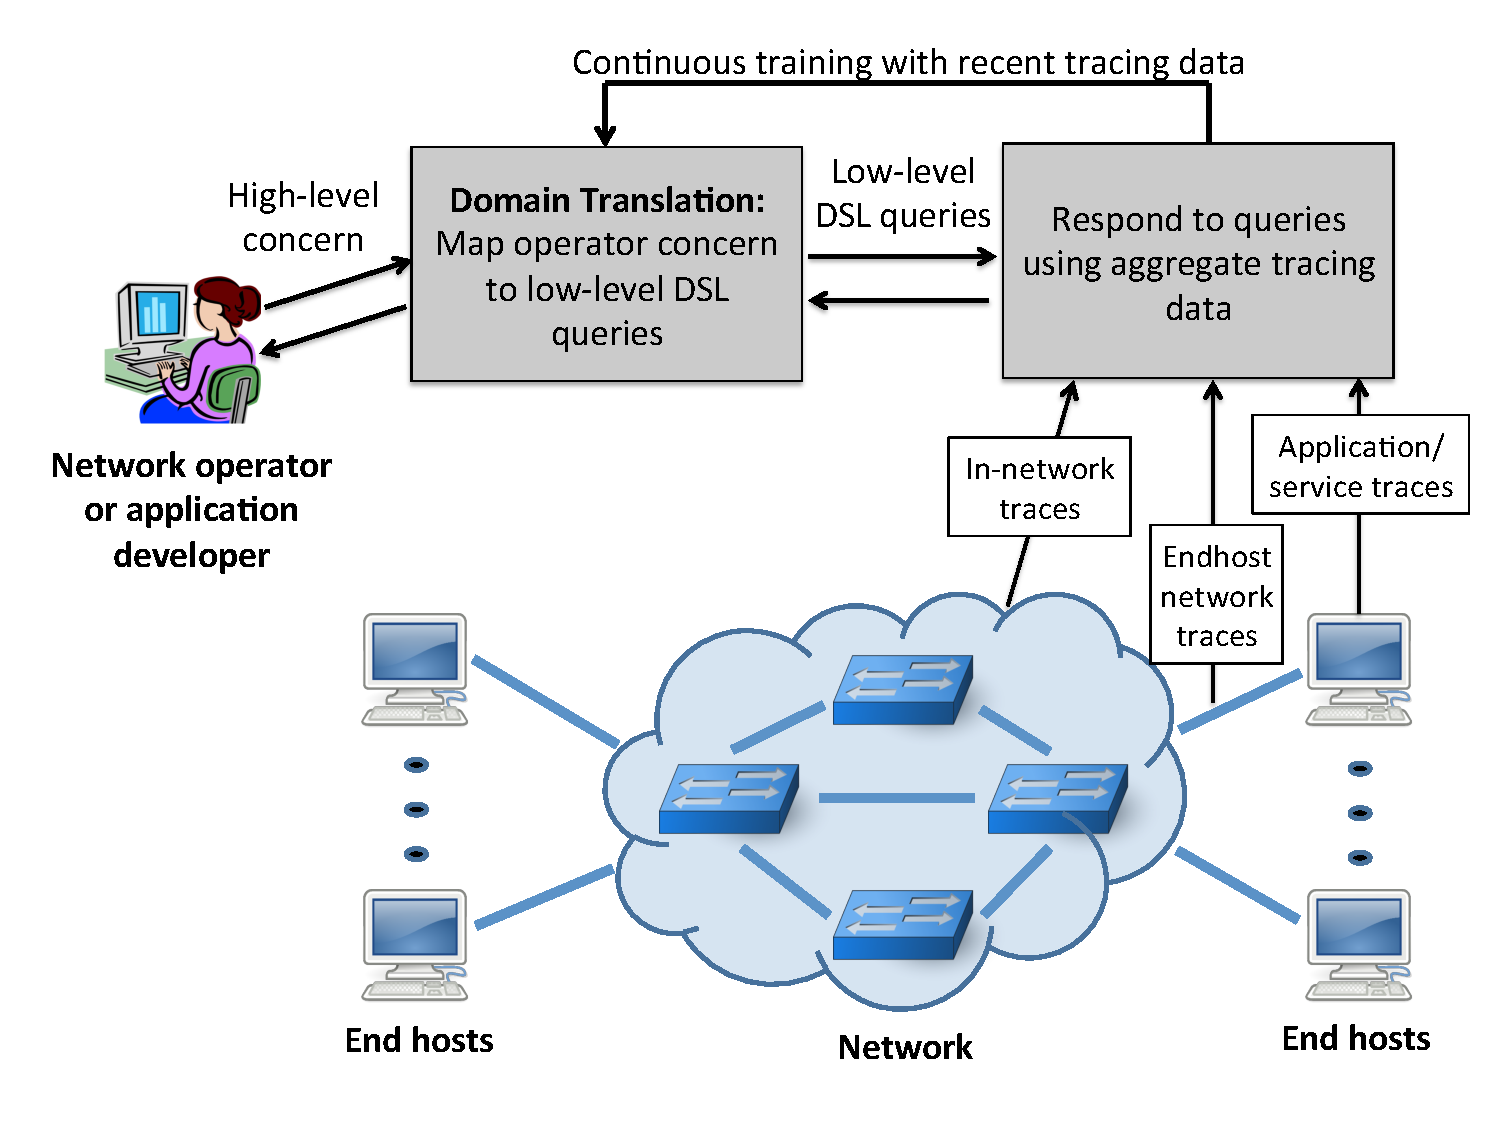
\includegraphics[width=0.7\textwidth]{tracing_figure.pdf}
\caption{Overview of our proposal to automatically bridge the gap between
operator/developer concerns and low-level tracing systems.}
\label{fig:overview}
\end{figure*}

In this proposal, we seek to bridge the gap between low-level debugging systems
and high-level operator concerns. In particular, our aim is to enable
developers to specify high-level concerns and automatically receive actionable
responses; the process of converting high-level concerns to DSL queries
encompassing application, endhost, and in-network debuggers will be automated
and hidden from developers and operators. Mapping high-level concerns to DSLs
can be done in one of two ways: 1) using tracing data which was collected
during the execution in question, or 2) assuming that all possible tracing data
is available. The former can use already collected data to provide a fast
response, but may restrict the set of possible DSL queries, potentially
affecting the response quality. In contrast, the latter approach isolates DSL
query generation from the available data, ensuring that the optimal queries are
considered; however, collecting the necessary data may be challenging as
execution environments are difficult to reproduce. We plan to explore this tradeoff
in more detail using concrete environments and real tracing data.

With either approach for generating DSL queries, a key challenge is to figure
out how to partition a potentially ambiguous high-level concern into the
appropriate DSLs. Prior systems have attempted to partition program logic
across different network domains~\cite{snap,maple}. However, these systems are designed
to receive well-formed inputs (often expressed with a separate DSL), and
partition logic across domains whose relationships are well understood (i.e., the
control plane and the data plane). In contrast, our proposal may be presented
with loosely-formed, high level concerns. In addition, we must map those
concerns to cooperative DSL queries across environments that are largely dynamic
and have been mostly treated in isolation to date.

To overcome these challenges, we propose two solutions. First, we plan to
employ Natural Language Processing techniques to bridge query abstraction
levels by mapping high-level operator concerns to DSL queries.  Second, we will
use tracing data collected at each point in the ecosystem (i.e., applications,
endhosts, and networks) to generate a model which relates low-level operations,
tracing data, and DSL queries across domains. Given the dynamic nature of the
end-to-end environment in terms of workloads, configurations, and available
data, we propose that each component is continually trained to update its model
with the latest tracing data. For example, training can use techniques like
LSTM to prioritize recently observed tracing data without forgetting past
(potentially sporadic) events~\cite{concode}. Figure~\ref{fig:overview} depicts
our proposed workflow.

Several properties of modern networks and distributed systems complicate this
vision. First, how can we support broad sets of loosely-formed queries? Prior
systems have attempted to automatically parse trouble tickets using NLP
techniques based on fixed keywords and input structures~\cite{netsieve}. In
order to support arbitrary queries from each part of the ecosystem, we plan to
develop models which relate keywords in each domain based on causal actions
observed in the collected traces.  Second, how can we collect sufficient
training data to cover the wide range of possible developer queries.  In
addition to training with actual snapshot data from prior execution and bug
reports, we plan to generate synthetic training data to highlight potential
issues (e.g., resource contention, race conditions, etc.).  Third, prior
systems have shown that collecting comprehensive tracing data at any one part
of a networked system poses scaling challenges, both for storage and
processing~\cite{pathqueries,demi}. Our proposal requires the aggregation of
tracing data from each part of the ecosystem. Because the importance of
collected data is most effectively considered in aggregate, we must develop
efficient pruning strategies that can scalably collect the important tracing
information without sacrificing insights.  Fourth, how can we handle
information gaps in the ecosystem due to privacy concerns over tracing data or
lack of administrative cooperation? Our models must be robust to varying
amounts of contextual data and misreported tracing data.

%In light of these challenges, we plan
%to keep the developer in the loop of the query generation process. In this way,
%developers may be able to provide additional information to tune intermediate
%representations that they still have familiarity with.

Prior work has proposed using machine learning for classification to associate
network-specific queries with tracing data from single
machines~\cite{netpoirot}. Our proposal differs from these approaches in two
key ways. First, we propose using machine learning in part as a language
translation tool, connecting the abstract, high-level developer language to the
low-level, structured query languages that existing tracing systems support.
Debugging systems have continually tried to raise the level of abstractions for
queries and user interfaces. 
% However, in order to go the next step and connect
% every part of the ecosystem, we believe that tackling the unstructured concerns
% of operators is the next challenge. 
Second, our proposed model that relates DSL
queries (and the corresponding tracing data) is not restricted to a single
machine that is controlled by one administrative entity. Instead, we plan to
merge data and DSL queries across different combinations of applications,
machines, and networks, in order to accurately respond to high-level developer
concerns with actionable suggestions.





\subsection{From Configurations to Policies: Extending Network Verification}

\paragraph*{Tool:} (Challenge C5, C7, Govindan, Millstein, Tamir, Varghese). A network architect must either map configurations at routers to a network policy ({\em verification}) or map a network policy to configurations at routers ({\em synthesis}) ({\bf S5}).

\paragraph*{Science:} Past work in network verification is unscalable or makes assumptions that limits its applicability; we will develop general approaches to these problems such as {\em stepwise refinement} and {\em network specific
data mining} to find bugs without specifications. We will also develop new algorithms to compactly encode the
{\em semantic difference} between two routers.

\paragraph*{Approach:}

Together with colleagues, we have helped pioneer the science of configuration verification (Header Space Analysis~\cite{hsa}); built tools for exhaustive data plane~\cite{hsa,netplumber,nod} and control plane~\cite{batfish,era} verification; and applied the idea of automated testing to data planes~\cite{atpg}.  In this thrust, we seek to improve the scalability of these tools and design missing pieces that prevent their application to a broader set of verification and synthesis problems in networking.

We propose new directions for verifying the data plane (the flow of data packets) and the control plane (the flow of routing packets).

{\em 1. Finding Bugs without Specifications:} It has now become standard practice to use formal methods and ``prove'' that the existing router configurations work correctly across all packets for both data plane (e.g., Veriflow~\cite{veriflow} and HSA~\cite{hsa}) and control plane (e.g., ERA~\cite{era}, ARC~\cite{arc}, and Minesweeper~\cite{minesweeper}).  However, this approach requires some form of specification to check the router or network model against.  In our experience, such specifications are often missing, wrong, or at best partially correct (basic beliefs
like ``Customer Machines should reach DNS'' are often correct~\cite{nod} but are only {\em partial} specifications). This is possibly because networks are managed by multiple operators, and there is also much legacy code in configurations that current operators do not understand but are scared to change.  This begs the question: can we find bugs without a specification?

The field of unsupervised learning and data mining suggests that one could {\em cluster} the set of routers in an operational network into partitions that we might term {\em roles}, confirm that roles are meaningful by looking for substantial agreement  between routers in a role, and finally spotting bugs as {\em anomalies} where some routers differ in some way from the majority of routers in the role.  We tried
straightforward approaches to clustering using off-the-shelf techniques like {\em k-means} and {\em Hamming distance} metrics, but failed to produce meaningful clusters despite tinkering with parameters.

This has led us to invent new {\em network specific clustering} algorithms. Note that the work in network verification such as Veriflow~\cite{veriflow}
and HSA~\cite{hsa} was able to scale because they exploited the structure of networks to scale verification beyond the limits and limitations of 
conventional verification tools like SAT solvers and symbolic execution applied blindly to the networking domain.  In the same way,
we believe that clustering and data mining must be rethought to exploit the structure of the network domain.

Consider, for example, the following network specific clustering that we find works quite well in practice.  We start with the
observation that most names assigned to routers in organizations are meaningful.  In UCLA, for example, a router
could be named br1.boelter.floor1, where the ``br'' stands for border router, and ``boelter'' is a building name. We have seen
similar behavior in other universities and corporations.  Thus, we divide the name into lexical tokens separated
by delimiters (such as punctutation while ignoring the numbers).  We then evaluate how meaningful each combination of tokens is as a role.  We use statistical techiques to evaluate the strength of each role as a hypothesis.  Once we find a good role partition (measured by substantial agreement in some precise sense between routers in a role), we then look for bugs as deviant configurations~\cite{engler} within each role.   

A nice feature of the above approach is its generality:  any clustering approach can be used, and statistical measures guard against poor choices.  This means that we can experiment with many different clustering algorithms and potentially employ combinations of them.  The name-based clustering technique described above is based on the reasonable assumption that human operators assign router names based on some implicit semantics.  However, not all networks employ a meaningful naming scheme, and even those that do are often not perfectly consistent.  As an alternative,
we have also investigated a role definition based on distance from the border of the AS: the nodes that interface directly with external ASes constitute one role, the nodes one hop away from those nodes constitute another role, etc.  
Our preliminary work with these approaches has identified new bugs that earlier technologies did not.  Our grant plans to flesh out these preliminary ideas, evaluate them scientifically on a much larger set of networks, and make the tools available publicly. 

{\bf 2. Synactic and Semantic Differences:} How can we tell whether a role is meaningful? For example, in UCLA it turns out that the pure router type (e.g. ``br'' for "border") is not sufficiently meaningful but the combination of type and building (e.g., ``br.boelter") is.  We measure goodness of a role by measuring the syntactic or semantic similarity of routers within the same role. A simple syntactic  check for example is to check for similar definitions, e.g., of DNS servers.  An anomaly then occurs when ``most'' (measured by a threshold) routers in a role have the same DNS server but a few do not.  

A more profound difference is to measure the semantic difference in terms of forwarding behavior of two routers across corresponding interfaces (e.g., upwards towards the ISP).  Existing network verification can verify that two routers are semantically equivalent, but if they are not equivalent only a single counterexample packet is produced~\cite{minesweeper}.  We have invented a new polynomial time algorithm that uses this existing technology as a subroutine in order to obtain the exact set of destination prefixes on which the two routers' behavior differs.  In addition to its use for partitioning nodes into roles, this algorithm could be used in any setting where it is useful to exactly characterize the differences between two nodes.  

Roughly the semantic difference algorithm is as follows.  Assume we are looking for the set of all destination prefixes that
are treated differently by two given routers.  We start by branching on prefixes that start with a 0 and those that start with a 1.  For each prefix $P$, we
ask Minesweeper~\cite{minesweeper} whether the two routers treat all destinations matching $P$ equivalently.  If Minesweeper finds they are equivalent, then we are done.  Otherwise, if there is {\em no} destination matching $P$ that the routers treat equivalently, then we return $P$.  Otherwise, we branch further, adding one more bit to the prefix $P$.

% \begin{verbatim}
% FindAllDiffs (R1, R2, P)  //* find all differences between router R1 and R2 for Destination addresses starting with Prefix P
%   If (For all addresses X that satisfies Prefix P, R1 and R2 have similar behavior) // Minesweeper call
%           return; //no differences
%   Else If (For all addresses X that satisfies Prefix P, R1 and R2 have differing behavior) // clever Z3 call invented by Alan
%            Print (P); //everything in P is a difference
%            return;
%   FindAllDiffs (R1, R2, P0); //recurse on P0
%   FindAllDiffs (R1, R2, P1); // recurse on P1
% \end{verbatim}

We have found that while the set of prefixes produced is fairly compact, one can compress further by using a bottom
up dynamic programming algorithm to also exploit the fact that many sets of prefixes can be compactly expressed
in a difference-of-cubes notation~\cite{hsa, nod}.  The algorithm walks the subtree of prefixes bottom up, evaluating the
costs of the two notations (positive form and difference form) to find the minimal representation.

{\em 3. Stateful Verification via Stepwise Refinement:} Stepwise refinement dates back to Dijkstra and Wirth~\cite{wirth}. With Ryzhyk~\cite{leonid}, we recently introduced refinement-based network programming as an intermediate stance between network verification (the user provides all configurations, the tool verifies) and synthesis (the user provides a specification, the tool synthesizes).  Instead, the user interacts with the system at each level of refinement to design and prove correctness of that level.
%
Step-wise refinement is especially promising because it may provide a way to address one of the major limitations of current tools: they cannot model stateful devices. In practice networks maintain state for several reasons (security, congestion control). However, if a router can  no longer be modeled as a function on a single packet but rather as a function on sequences of packets, the state space becomes very large~\cite{mooly-tacas16}.  We hypothesize that step-wise refinement can escape this verification conundrum analogous to way a theorem prover can outperform a model checker if the user specifies high-level invariants.   We will work with Ryzhyk at VMWare to verify Network Function Virtualization (NFV) devices such as Google's Maglev load balancer~\cite{maglev}. 

Moving to synthesis we plan to work on:

{\em 4. Synthesis for Rural Networks:}  We have already proposed extending the work in Propane on control plane synthesis from data center networks to ISPs in an NSF Medium grant (Butane~\cite{butane}) with David Walker at Princeton.  While Butane {\em extends} Propane to cover more use cases, in this grant we {\em simplify} Propane to handle simpler rural networks such as WISPs~\cite{barathwisp} (with PI Barath Raghavan). WISP operators in Africa, India, and rural US will not learn a new network policy language but may be willing to try a phone-based UI that verifies connectivity and suggests configuration changes in response to common events. This type of synthesis adds challenges not seen in the data center context, as the topological challenges are external (e.g., terrain/line of sight, spectrum, power, etc.) and the resources available to the operator are limited~\cite{zyxt18}.
%\jnf{Phone-based UI? Seriously? These operators don't even have access to a desktop or laptop machine?}

We do not propose any work in configuration synthesis in this grant because we have already proposed generalizing the work in Propane~\cite{propane} on control plane synthesis in an NSF Medium grant led by David Walker at Princeton that is joint with Millstein and Varghese. 

\subsection{From Configurations to Tests: Creating Automated Network Tests}

\paragraph*{Tool:} (Challenge C5, C7, Millstein, Tamir, Varghese). Many vendors including Microsoft and 
Google have created VM frameworks to test routers and their configurations, because verification only verifies a {\em model} at  each router.  Unfortunately, these frameworks require
the tester to manually supply tests.  Instead, we suggest automated testing of network routing.

\paragraph*{Science:}  Inspired  by our earlier work ATPG~\cite{atpg} for testing data planes and software tools for automated test generation (e.g., KLEE~\cite{klee}, we will automatically generate test {\em routing announcements} and emulate on UCLA and USC topologies.

\paragraph*{Approach:}

Unlike KLEE, ATPG gets away with a much simpler algorithm based on set cover compared to say KLEE or DART because (in bug-free networks) there are no cycles (although network verification can and should check for such cycles first before applying such methods): hence the state space is finite (though large).   KLEE and DART have a more complex set of heuristics to search the infinite 
space of executions caused by programs that can have loops.   

However, BGP and OSPF provide
an interesting intermediate ground; unlike loop-free data packet forwarding, BGP announcements can be batted back and forth before they converge
and simple set cover is unlikely to work.   On the other hand, most commonly used forms of BGP are not as complex as arbitrary code.
Thus we seek intermediate methods that are tailored to networking without the complexity and generality of
say KLEE or DART (which must handle arbitrary code).   The intellectual component of this grant largely arises from navigating this tradeoff space.  

While this approach is inspired by software testing, we are also inspired by hardware testing which has a prolific literature.  PI Tamir has worked in the field of computer architecture and will pursue the connections between hardware notions of testability and coverage, and networks.  [[Yuval add some stuff here]]
showing how 




\subsection{From Network Queries to Router Commands: Performance Monitoring}

\paragraph*{Task:} (Challenge C9, Foster, Weatherspoon). After designing a network, a {\em network operator} must monitor the network for performance problems such as traffic bursts and unexpected failures ({\bf S7}).

\paragraph*{Science:} Past work~\cite{perl1994performance} allows operators to specify higher level performance invariants for multiprocessor systems; we will generalize to allow performance assertions for networks.

\paragraph*{Approach:} We will develop a high-level query language and distributed run-time that exploints features provided on next-generation network hardware (Section~\ref{sec:compiler}) but also for existing IP networks. It will map network-wide performance queries down to commands that can be executed on individual routes and switches. This challenge is similar to mapping network programs discussed previously, but adds several new dimensions, beacuse queries are typically quantitative and can often be answered only approximately. For example, we might implement a query that monitors a single flow by installing  forwarding rules that tag and count matching packets, or one that computes the global traffic matrix query by aggregating counters polled from all devices at the edge~\cite{srinivasan}.

While several existing systems~\cite{srinivasan,ndb,netsight} develop some basic machinery for answering queries, they are point solutions in that they only offer limited expressiveness and require SDN switches.  We believe we can generalize Perl's notion of performance assertions that she used  to monitor a multiprocessor system\cite{perl1994performance}  to existing IP networks and to newer P4 switches, and use them to  concisely express and efficiently evaluate ``difficult'' queries such as identifying bottlenecks or estimating available bandwidth.

We plan to compile performance assertions to existing router commands to poll router counters and logs, using a RegEx engine to correlate information across multiple devices. Before a router crashes or reboots, it will attempt to write a message to a \texttt{syslog} file. Hence, a query to find all routers that have port flapping events in the last hour, we can use a performance assertion about the rate of flap events, which can be computed from the \texttt{syslog} files for all routers. In addition to targeting existing routers, we also plan to take full advantage of emerging platforms such as P4, a goal we share with~\cite{srinivasan}. 

%The key insight is that we apply programming language techniques, experience, and expertise designing approaches for network-wide abstractions and associated compilers and tools with dataplane programming languages such as P4 and next-generation dataplane hardware such as enabled by dataplane programming languages.  Together, we create an approach for performance monitoring automation.

\begin{comment}
In our vision, network operators specify performance properties using high-level, network-wide abstractions (e.g., regular paths, logical predicates) which are automatically compiled  into run-time monitors (e.g., Syslog monitors, SNMP queries to router counters) that continuously check the healthiness of the network and alert operators upon violation.  

Our approach is inspired by performance assertion checking designed for multi-threaded programs~\cite{perl1994performance}, but tailored for networks that have stringent performance requirements (line rate) and limited resources (computation and storage).  The key insight is that we apply programming language techniques, experience, and expertise designing approaches for network-wide abstractions and associated compilers and tools with dataplane programming languages such as P4 and next-generation dataplane hardware such as enabled by dataplane programming languages.  Together, we create an approach for performance monitoring automation.


%Example Performance Queries\newline
%  Congestion,
%  Latency,
%  Available Bandwidth,
%  Load Balancing,
%  Blackholes,
%  Stability
%
%Performance Monitoring Compilation
  
\paragraph*{Research Challenges.}
%
%Challenges: Part of broad challenges at start of grant. Manual effort today 
%Solution Idea:  Inspired by PL ideas in keeping with grant
%
Challenge for performance monitoring and debugging automation are three fold.  First, designing a performance monitoring language and run-time requires balancing tension between ``per-flow'' and ``network-wide'' properties.  Second, instantaneous snapshots of the network, which are required for testing performance properties, are not possible.  Instead, performance monitoring will require concepts from distributed systems such as consistent cuts.  Finally, high line rates and limited hardware, storage, and computation inside the network, may require sampling and approximation.

  
\paragraph*{Scientific Impact.}
%
If successful, this work represents a transformative step for performance monitoring and debugging in networks.  It raises the level of abstraction for performance monitoring involving quantitative and global properties.  It takes a high-level specification of network-wide performance properties and compiles them to low-level, distributed, and continuous monitoring checks.  It automates the entire process of performance monitoring, which is significant.  Finally, the broader impact will make networks much more reliable.

\end{comment}


\begin{comment}
\paragraph{Other Related Prior Work.}
%  
Examples\newline
(1) Perc (SOSP 2013)

Describe data to log using intervals and metrics

Specify performance properties using assertions formulated in terms of simple aggregation operators

{\em Provides abstractions for specifying which data should be collected from a distributed system and which properties should be checked}

Intervals
\begin{verbatim}
  interval Read = s: StartRead, e: EndRead
  metrics time = ts(e) - ts(s)
  end Read
\end{verbatim}

Performance Assertion
\begin{verbatim}
  assert {&r : Read : r.time <= 10ms} 
\end{verbatim}

(2) Path Queries (NSDI 2016, SOSR 2016)\newline
Specify which packets to monitor using regular expressions

Implementation tracks state of query automaton using switch forwarding rules and counters

Felix analyzes configurations to implement monitoring at edge, reducing complexity and churn in core

{\em Path queries provide declarative abstractions for expressing network-wide path queries… but limited to single-packet properties}

Regular Expression
\begin{verbatim}
  p1 = in_atom(scrip=H1 & switch=1) ^ out_atom(switch=2 & dstip=H2)
  p2 = in_atom(switch=1) ^ in_out_atom(tru, switch=2)
\end{verbatim}

Automation
\end{comment}


\subsection{Making Routers Observable and Controllable:  Router Boundary Scan}

\paragraph*{Task:} (Challenge C9, Netravali, Tamir, Varghese).  Many faults in routers are caused not by configuration 
problems but by microde or hardware bugs that are hard to isolate because it is difficult to send test inputs to 
operational routers to diagnose the problem. Imagine that we could send a  Voice over IP packet between two routers in the middle
of the network to test whether its being delayed in a queue at either router.  Or to send a BGP annoucement to only one router to
manupulate its Routing Table?  Imagine that we could also observe the state of the routers after each such packet.  Then routers
would become {\em controllable} and {\em observable}.

\paragraph*{Science:} Past work~\cite{jtag} in {\em hardware boundary scan} (implemented in a standard popularly known as JTAG) allows hardware modules (e.g., chips) to be sent arbitrary test input (Figure~\ref{rtagfigure}) and the output 
fron the same module to be read out by the tester without having physical wires from the tester to each chip.  Inspired
by this idea, we propose {\em router boundary scan} to allow a tester to send an {\em arbitrary packet} (e.g., an application
packet or even a router announcement) to an {\em arbitrary} router to be sent out on an arbitrary interface, and having the 
router hardware snapshot state at the receiving and sending ends that can be later collected by the tester.

\paragraph*{Approach:} If we consider a router as a module, we are looking to send arbitary test inputs to the router and
observe the results.  Software module testing is comparitively easy because we can typically isolate a software module in
a test harness.  However, in hardware, if the system is a board and the ``modules'' are chips, it is often difficult to find 
the right set of board inputs to send appropriate test signals to a specified chip.  Wires from the tester to each chip would
work but this would grreatly increase the number of pins.  Instead, in hardware boundary scan, (Figure~\ref{rtagfigure}) a few
 shared JTAG pins are reserved for testing and the test inputs is connected to a daisy chain serial network that reaches all
 pins.  The test input for say a chip $C2$ can then be shifted through the prior chips in the daisy chain network till it
 reaches $C2$.  A similar daisy chain network is used to collect the output from $C2$.
 
 \begin{figure*}[t]
\centering
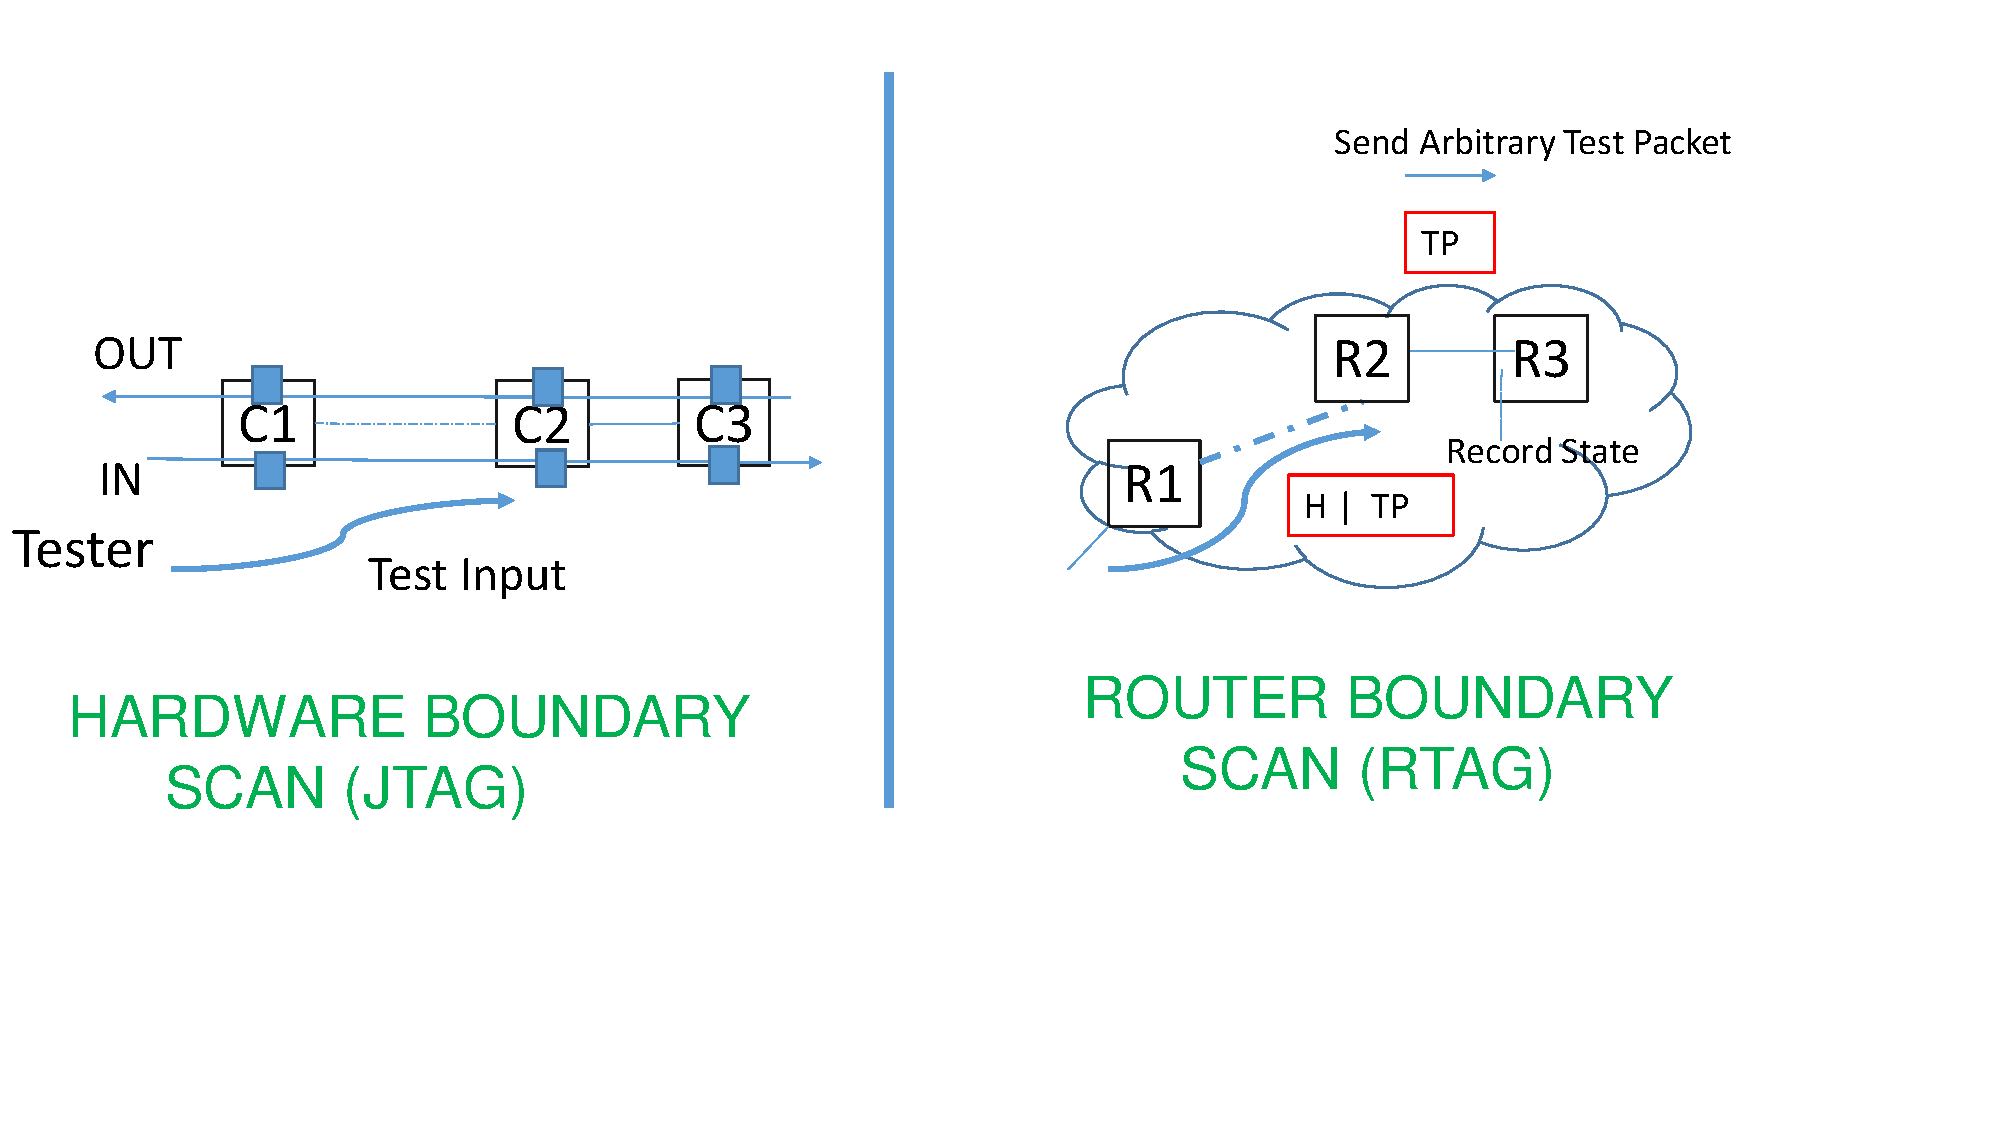
\includegraphics[width=0.7\textwidth]{RTAG.pdf}
\caption{Overview of our proposal to automatically bridge the gap between
operator/developer concerns and low-level tracing systems.}
\label{fig:rtagfigure}
\end{figure*}

 Inspired by this, we propose a new router boundary scan mechanism (RTAG for Router Target Action Generation) where an
 external tester can send an arbitrary packet ({\em TP}  on the right of Figure~\ref{rtagfigure}) to an arbitrary router ($R3$) 
 by encapsulating it (using say IP in IP encapsulation) to $R4$ together with control information that specifies which interface
 it must be sent on.  Before sending the test packet {\em TP} the tester ``arms'' the other end of the interface (e.g., $R3$) to
 detect this test packet using a prespecified pattern detection predicate.  Just as in JTAG, we propose that every router add
 new hardware to snapshot state (e.g., time sent/received, queue sizes) on sending/receiving {\em TP} which can later be collected by the
 tester.
 
 We believe that Router Boundary Scan can help real time detection of a number of hard to isolate phenomena we have observed
 in data centers including hardware and microcode bugs, and mysterious packet losses.  Further, we believe this can be combined
 with the network system debugging described in Section~\ref{ravi} to go from operator logs to tester queries to isolation to particular
 routers.  From discussions with Cisco's Tom Edsall\footnote{the chied designer of Cisco's Catalyst Route and their latest Data Center routers}, it appears that such a mechanism is not available in any current router but is feasible to add. Edsall (see letter) is willing to work with us to refine this scheme so
 that its hardware implementation is feasible.
 
 Our proposal differs from existing work in testing like ATPG~\cite{atpg} which relies on external data packets to test routers (and hence
 has limited and only indirect controllability), hardware schemes like INT~\cite{int} and Maple~\cite{maple} which do not allow the sending of an arbitrary packet
 to an arbitrary router (but can collect specified state such as queues, this enhancing observability not controllability), and schemes such
 as Postcards (that record all the state seen by a given data packet (also enhancing observability and somewhat expensive).  Closest to our
 work is the Directed Probes mechanism implemented in Everflow~\cite{everflow} but Evrerflow uses commodity switches and so 
 cannot do a general state snapshot on sending and receiving, and thus while controllable and observable separately, Everflow 
 is not {\em both} controllable and observable as RTAG is.

The lazy collection approach in Router Boundary Scan can also be generalized to do in-band testing of an application's traffic to simulate ``Stepping''
into and out of a router as in a software debugger.  The idea is that application packets can sometimes set a Tracing bit which causes state to
be snapshotted at the router as the packet enters and leaves, but the application packet speeds through the router.  The tester then lazily collects this
snapshot state at each router using some form of packet ID (as in IEEE 1488) and then software can allow the operator to step through each router
in the path retrospectively to examine the time of arrival and queue sizes when the application packet arrived.

We propose to implement Router Boundary Scan and Router Stepping in a NetFPGA testbed and use it to diagnose injected faults and to integrate
it with the Application Level debugging described in Section~\ref{ravisec}.
 
 
 
 


\subsection{From Failure Logs to Models: NLP for Extracting Cause-effect Patterns}

\paragraph*{Task:} (Challenge C9, Govindan, Netravali, Varghese)  
Operators need techniques to analyze failures to prioritize
network engineering and design decisions (\textbf{S9}).

\paragraph*{Science:} Relatively little research in Natural Language
Processing has addressed the extraction of cause-effect relations in
text. We will develop natural language learning methods that capture
the linguistic patterns that denote causal relations that appear in
network failure reports.  Our research will help us suggest what
\emph{minimal} (because we believe it is unlikely that operators will
adopt completely structured reporting) descriptions can be added
to logs and failure reports to enable richer analyses.

\paragraph*{Approach:}  At four or five nines availability, cloud providers can afford only a few minutes of
outages per month~\cite{rameshgoogle}, and even using NDA tools, it is likely that failures will happen.  Today, cloud operators maintain logs that describe
changes to the network and document analyses of failures.  These logs are 
examined manually today~\cite{rameshgoogle}. We propose
to exploit these logs to automatically (a) categorize root causes of
failure, and (b) develop a succinct abstraction (a failure
\emph{cause-effect} graph) to represent each failure. 

In preliminary work, we performed a detailed manual analysis of
unstructured text in post-mortem reports of over 100 high-impact
failure events within Google’s network \cite{rameshgoogle}. Here, we
instead propose to use Natural Language Processing to develop failure
abstractions. It will take new science in Information Extraction,
Discourse Analysis and Domain Adaptation to develop natural language
learning methods that accurately and robustly capture the {\it
  linguistic patterns} for {\it causal relations} that appear in
network failure reports.
%
Linguistic patterns for causal relations, for example, can appear in
compound nouns ({[{\sc effect}]\textsubscript{NP}} {\it incident}), as
subject-object pairs ({[{\sc effect}]\textsubscript{SUBJ}} {\it was
  triggered by} {[{\sc cause}]\textsubscript{OBJ}}),
%e.g.\ {[the incident]\textsubscript{EFFECT}} {\it was triggered by}
%{[a guest OS rollout]\textsubscript{CAUSE}})
or across sentence boundaries, with or without intervening discourse cues
like ``as a result" ({[The guest OS rollout]\textsubscript{CAUSE}} was
applied to Cluster B at 10:10am. {[Connectivity was lost]\textsubscript{EFFECT}}
at 10:11am.).

We believe that root-cause categorization is amenable to standard \emph{text
  categorization} techniques~\cite{Sebastiani:2002:MLA:505282.505283}:
  given a bag-of-words representation of a post-mortem report failure
  {\sc discussion}, supervised classification methods
(e.g.\ SVMs~\cite{Joachims1998}, maximum entropy
classification~\cite{Pang:2002:TUS:1118693.1118704}, deep averaging
networks (DANs)~\cite{Iyyer:Manjunatha:Boyd-Graber:Daume-III-2015})
can be applied to classify the text according to
the type of the root cause it describes.  The challenge here will be to
develop sufficient training data for accuracy. We propose to use
active learning methods
\cite{cohn1996active,mccallumzy1998employing,tong2001support}
that select the most useful
examples to add to the training set in each iteration. Finally, to
discover new root-cause categories, (an instance of ``concept drift''
\cite{widmer1996learning,klinkenberg2000detecting}) we propose
human-in-the-loop clustering with constraints \cite{wagstaff2000clustering,wagstaff2001constrained,cohn2003semi,Mierswa:2006:YRP:1150402.1150531}:
cluster the new and existing post-mortem reports
and ask a networking expert to inspect the result, looking for
partitions that contain network failure events that fall outside the
current set of known root causes.

Beyond root-cause categorization, a useful abstraction that succinctly
summarizes a single failure is a {\it cause-effect failure graph},
which relates failure causes (software or hardware components) to
observed effects. This abstraction will permit network operators to
analyze, across many failures, which components fail most often and
under what conditions, enabling them to prioritize resources for
reliability engineering and network re-design. From an NLP point of
view, the extraction of cause-effect graphs is most easily viewed as a
task in {\it information extraction}
\cite{cardie1997empirical,freitag2000machine,sarawagi2008information}
in which limited kinds of domain-specific semantic content (i.e.,
network failure causes, locations, effects) are extracted from
unstructured text (i.e., post-mortem report {\sc discussion}s), and
transformed into structured formats (i.e., a cause-effect graph)
suitable for analysis. Extracting cause-effect relations remains an
open problem in NLP.  We propose to build on research
\cite{kozareva:2012:TextGraphs-7,oh-EtAl:2013:ACL2013,CAtoCL:2014,mirza-tonelli:2014:Coling,hidey-mckeown:2016:P16-1}
in causal relation identification to develop domain-specific
techniques that can identify both within-clause causal relations,
inter-clausal and inter-sentential expressions of causality, as well
as the coreferential relations among the entities, states and events
involved.

Some of these approaches to NLP for network failure analysis were developed with Claire
Cardie at Cornell, an NLP Expert.  We also plan to consult Kai-Wei Chan, an NLP expert at UCLA.


\iffalse
%%% Claire:  from preproposal review
%% The portion of the proposal that involves text analysis and NLP
%% was not well-integrated with the rest of the proposal: in the
%% full proposal, its necessity to the larger vision and its
%% integration with the other areas could be more fully developed,
%% or perhaps it could be separated out into another proposal.

%% CAN NDA SUPPLY AUTOMATED TOOLS FOR DIAGNOSING FAILURE ROOT CAUSES AND LOCALIZING FAILURES?
Maintaining the highest levels of availability for content providers
is challenging in the face of scale, network evolution, and
complexity. With promised availability rates of 99.99\%-99.999\%,
however, network failures cannot exceed a few minutes or seconds per
month.  Google’s internal availability target for user-facing traffic,
for instance, is no more than a few minutes downtime per
month~\cite{rameshgoogle}.
%
It is critical, therefore, to make progress on the
development of automated tools that can inform network design and
analysis.
% for NDA to supply automated tools for
% diagnosing failure root causes and localizing failures.
%
Current industry practice requires operators to maintain logs that
store informal records about changes made to topologies and
configurations, as well as post-mortem analyses of failures.  We
propose here, to exploit these logs as a key source of information for
developing the next generation of NDA tools.

In preliminary work, for example, we performed a (manual) detailed analysis
of the post-mortem reports of over 100 high-impact failure events
within Google’s network \cite{rameshgoogle}. From the
reports, we determined the root cause(s) of the failure
as well as its specfic effects on network components and performance,
allowing us to quantify several dimensions of availability
failures. In particular, we found that failures are evenly distributed
across different network types and across data, control, and
management planes.  In addition, a large number of failures happen when a
network management operation is in progress within the network.  This
failure analysis, in turn, informed the development of new design
principles for high availability, including using defense in depth,
maintaining consistency across planes, failing open on large failures,
carefully preventing and avoiding failures, and assessing the root
cause quickly.

%% From Claire:  from preproposal review...need to address the following
%% somewhere. Maybe in the next paragraph?
%% ``Using NLP for mining current cloud logs is quite promising. It
%% is not very clear, however, whether the generation of logs
%% itself should be standardized and optimized to reduce the
%% difficulty for such mining. It would be good to have some
%% discussions in this aspect.''

Unfortunately, the manual analysis of each post-mortem report is
painstakingly slow and the development of useful and robust design
principles necessarily requires the analysis of dozens, or better yet,
hundreds of failure post-mortem reports.  So, while the results of our
study were fruitful, the current process does not scale.
%
Fortunately, much progress has been made in recent years in the field
of natural language processing (NLP) where methods for {\it text
  categorization}, {\it information extraction} and {\it cause-effect
  analysis} are especially relevant.  In the sections below, we
 describe plans for employing these and other methods from NLP and
machine learning (ML) for root-cause classification and the creation
of cause-effect failure graphs to support the continued development of
high availability network design principles.
    
\subsection{Root-cause classification}

\begin{table}[thbp]
  \centering
  \begin{tabular}{|c|l|} \hline
    Data & Hardware failures or hardware misconfiguration \\ \cline{2-2}
         & Control−plane network failure \\ \hline
    Management & Incorrectly executed management process \\ \cline{2-2}
               & Risk assessment failure \\ \hline
    Control & Routing misconfigurations \\ \cline{2-2}
            & Lack of consistency between control plane elements \\ \cline{2-2}
    & Device resource overruns \\ \hline
  \end{tabular}
  \caption{Hierarchy of failure event root causes.  The first level
    indicates which of the data plane (i.e.\ (hardware) components
    that how networks process traffic), control plane (i.e.\ software
    that determines how to set up the rules by which the data plane
    processes traffic) or management planes (i.e.\ network
    (re-)configuration by operators) planes was at fault. The second
    level provides the class of fine-grained root cause for the
    failure.}
   \label{table:root-causes}
\end{table}

In addition to the {\sc location} of the network failure, its {\sc
  duration}, {\sc impact on traffic volumes} and {\sc packet loss
  rates}, etc., a typical post-mortem report also includes an
unstructured {\sc discussion} of the root causes of the failure. To
quickly identify and classify the root causes, we propose the use of
standard {\it text categorization} techniques [refs]: given a
bag-of-words representation of {\sc discussion}, supervised
classification methods (e.g.\ SVMs [ref], maximum entropy models
[ref], deep averaging networks (DANs) [refs]) are applied to classify
the text according to the type of the root cause it describes.  To
start, we will employ the two-level root-cause hierarchy identified
in~\cite{rameshgoogle} and shown in
Table~\ref{table:root-causes}.

\paragraph{Evaluation.} We will evaluate the approach using leave-one-out cross-validation on
the 130 Google post-mortem reports that were annotated according
failure type in the \cite{rameshgoogle} study. To obtain usable
levels of performance, we expect to need additional training
data.\footnote{This is surely the case for neural network
  classification methods, but can also be an issue for non-neural
  approaches.}  For this we will annotate network failure reports from
\url{https://github.com/danluu/post-mortems}.  Further, to minimize
the amount of training, we propose the use of {\it active learning}
methods \cite{[refs]} that select the most useful examples to add to
the training set in each iteration (i.e.\ reports whose classification
the current model is least confident in).

\paragraph{Identification of new types of root causes.}  The categories of root causes for network
failure in \cite{rameshgoogle} is known to be incomplete --- it
covers about 70\% of the studied Google network failure.  In any case,
the set will certainly need to evolve over time as networking
technology changes.  As a result, we will also investigate approaches
for identifying new types of root causes.  Following existing ML
research of this phenomenon (sometimes referred to as ``concept
drift'') \cite{[refs]}, we propose human-in-the-loop clustering
(e.g. \cite{[refs]}): cluster the new and existing post-mortem reports
and ask a networking expert to inspect the result, looking for
partitions that contain network failure events that fall outside the
current set of known root causes.

\subsection{Cause-effect failure graphs}

\begin{wrapfigure}{r}{0.65\textwidth}
%  \footnotesize
%  \hspace{-3mm}
%  \includegraphics[width=0.65\textwidth]{cause-effect.jpg}
  \caption{Cause-effect Failure Graph Extraction}
  \label{fig:cause-effect}
\end{wrapfigure}

The construction of high availability design principles
in~\cite{rameshgoogle} required the manual analysis of the
post-mortem {\sc discussion}s that describe the hardware status
information and software outputs and bugs identified by cloud and
network operators in their attempt to isolate failure symptoms and
root causes.  Specifically, the analysis determined the sequence of
EVENTS and STATES that {\sc cause}, or contribute to, a network
failure; their {\sc location impact} and {\sc time} of occurrence; and
the {\sc resulting effect}s.  Once identified, this information can be
concisely described as a {\it cause-effect failure graph}.\footnote{In
  additional (unpublished) preliminary work, we created a prototype to
  automatically extract network failure {\sc causes} from logs: The
  prototype employed the Stanford Parser \cite{klein-manning:2003:ACL}
  and an existing system, called NetSieve \cite{netseive:2013:nsdi}
  (based on classical rule-based IE methods), and found the outputs
  too low-level to be useful; hence, our move to the cause-effect
  graph representation proposed here.} The graph shown in
Figure~\cite{fig:cause-effect}, for example, indicates that the guest
OS rollout (from 2/8/14) together with the lack of an SLB (stream load
balancer) plugin on Cluster X in Datacenter A caused connectivity loss
(on 2/8/14).
%
It is the subsequent analysis of the cause-effect graphs from many
failure reports that will facilitate the construction of design
principles based on, e.g., which components are most likely to fail,
whether there are common failure patterns, under what conditions
(traffic, usage) the failures occur, whether there are early warnings
of failure.

From an NLP point of view, the extraction of cause-effect graphs is
most easily viewed as a task in {\it domain-specific information
  extraction} in which limited kinds of domain-specific semantic
content (i.e., network failure causes, locations, effects) is
extracted from unstructured text (i.e., post-mortem report {\sc
  discussion}s), and transformed into a structured format (i.e., a
cause-effect graph) suitable for populating a database.  There has
been extensive research in the field of information extraction over
the last 20+ years \cite{[refs]}, including work to identify named
entities \cite{[refs]} and fixed sets of the binary relations they
occur in (e.g., X {\sc located-in} Y, X {\sc married-to} Y, X {\sc
  part-of} Y) \cite{[refs]} as well as the more complex undertakings
of event extraction (e.g., identify the type of event, its location,
time, participants, outcomes, affected entities) \cite{[refs]} and
opinion extraction (for each expressed opinion or sentiment, identify,
e.g., its opinion holder, target, polarity (positive, negative),
intensity) \cite{[refs]}.

There has been much less work done on the extraction of general
cause-effect information from unstructured text; nevertheless, a
number of approaches have been proposed in recent years (see, for
example, \cite{CAtoCL:2014}) including rule-based methods (e.g.,
\cite{bogel-EtAl:2014:CAtoCL}), ML-based classification (e.g., for
determining causality between events
\cite{mirza-tonelli:2014:Coling}), discourse-based learning approaches
(e.g., \cite{oh-EtAl:2013:ACL2013}) as well as associated research for
acquiring the necessary lexicons (e.g.,
\cite{kozareva:2012:TextGraphs-7}) and linguistic cues (e.g.,
\cite{hidey-mckeown:2016:P16-1}).  To date, however, the extraction of
causal relations remains an open problem in NLP.

We propose to build on the above research on causal relation
identification to develop domain-specific techniques for cause-effect
graph extraction that can identify both within-clause causal relations
(see S1 and S2), inter-clausal and inter-sentential expressions of
causality (S3), and the coreferential relations among the
entities, states and events involved:

\begin{quote}
S1: [The incident]$_{EFFECT_1}$ was triggered by [a guest OS
    rollout]$_{CAUSE_1}$ $\ldots$
     
S2: [The incident]$_{EFFECT_1}$ resulted from [a load
    balancer software update]$_{CAUSE_2}$ $ldots$ to [hardware
    clusters]$_{LOCATION_1}$.
       
S3: When [a guest OS rollout]$_{CAUSE_1}$ $\ldots$ was applied to
    [those clusters]$_{LOCATION_1}$, [connectivity was
    lost]$_{EFFECT_1}$ $\ldots$
\end{quote}

\noindent
Coreference relations are denoted via subscripts (e.g., ``the
incident'' of S1 and S2 is the loss of connectivity of S3).
Note that inter-clausal and inter-sentential causal relations can
be explicitly marked (e.g., via the discourse connective ``when'' in
S3 or denoted implicitly (as is the case for linking the
``connectivity loss'' in S3 with its cause described in the first
clause).
    
We will apply existing state-of-the-art methods for all subtasks:
classification-based learning methods for within-clause cause-effect
relation extraction [refs] and noun-phrase coreference resolution
\cite{[refs]}, neural network-based sequence tagging methods for
inter-sentential causal relation extraction \cite{[refs]}, sequence tagging
methods \cite{[refs]} for identifying network entities (e.g., ``load
balancer'', ``hardware clusters''), and Bayesian models for event
coreference resolution \cite{[refs]}.  In recent years, it has proven
effective to employ methods that {\it jointly} identify entities and
their associated relations \cite{[refs]}; as a result, we will focus our
investigation on these for cause-effect graph extraction.

All of the state-of-the-art techniques involve supervised machine
learning methods, which require annotated data for training.  And
while there exist data sets for each of the tasks described above,
none include text from network failure reports.  As a result, we
expect to need {\it domain adaptation} techniques that tranfer NLP
models trained on text from one domain (e.g., newswire) to perform
well on text from a very different target domain (e.g., failure
reports).  Because these techniques typically require at least some
annotated text from the target domain, we plan to use {\it active
  learning} \cite{[refs]} and new methods in the area of {\it data
  programming} \cite{[refs]} to create the labelled data sets quickly.

\paragraph{Evaluation.} We can evaluate performance on cause-effect
graph extraction on the Google data set of ~130 failure reports, after
annotating them manually with their associated cause-effect graphs. We
will use the standard performance metrics employed in information
extraction, measuring Recall, Precision and F-measure.
\fi


